\olchapter{sfr}{infinite}{Infinite Sets}

\begin{editorial}
This chapter on infinite sets is taken from Tim Button's \emph{Open
Set Theory}.
\end{editorial}



\olfileid{sfr}{infinite}{hilbert}
\olsection{Hilbert's Hotel}

The set of the natural numbers is obviously infinite. So, if we do not
want to \emph{help ourselves} to the natural numbers, our first step
must be characterize an infinite set in terms that do not require
mentioning the natural numbers themselves. Here is a nice approach,
presented by Hilbert in a lecture from 1924. He asks us to imagine
\begin{quote}
[\ldots] a hotel with a finite number of rooms. All of these rooms
should be occupied by exactly one guest. If the guests now swap their
rooms somehow, [but] so that each room still contains no more than one
person, then no rooms will become free, and the hotel-owner cannot in
this way create a new place for a newly arriving guest [\ldots
\textparagraph \ldots]

Now we stipulate that the hotel shall have infinitely many numbered
rooms $1$, $2$, $3$, $4$, $5$, \dots, each of which is occupied by
exactly one guest. As soon as a new guest comes along, the owner only
needs to move each of the old guests into the room associated with the
number one higher, and room~$1$ will be free for the newly-arriving
guest. 
	\begin{center}
		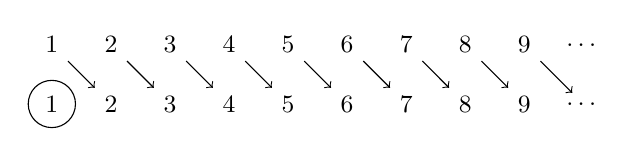
\begin{tikzpicture}[scale = .75]
		\foreach \x in {1, 2, 3, 4, 5, 6, 7, 8, 9}
		{
			\node (\x a) at (\x, 1) {\small{\x}};
			\node (\x b) at (\x, 2) {\small{\x}};
		}
		\node (dotsa) at (10, 1) {\small{\ldots}};
		\node (dotsb) at (10, 2) {\small{\ldots}};
		\draw[->] (1b)--(2a);
		\draw[->] (2b)--(3a);
		\draw[->] (3b)--(4a);
		\draw[->] (4b)--(5a);
		\draw[->] (5b)--(6a);
		\draw[->] (6b)--(7a);
		\draw[->] (7b)--(8a);
		\draw[->] (8b)--(9a);
		\draw[->] (9b)--(dotsa);
		\draw (1,1) circle (.4);
		\end{tikzpicture}
	\end{center}
	(published in \citealt[730]{EwaldSieg2013}; our translation)
\end{quote}
The crucial point is that Hilbert's Hotel has infinitely many rooms;
and we can take his explanation to define what it means to say this.
Indeed, this was Dedekind's approach (presented here, of course, with
massive anachronism; Dedekind's definition is from
\citeyear{Dedekind1888}):

\begin{defn}\ollabel{defn:DedekindInfinite}
A set $A$ is \emph{Dedekind infinite} iff there is !!a{injection}
from~$A$ to a proper subset of~$A$. That is, there is some $o \in A$
and !!a{injection} $f \colon A \to A$ such that $o \notin \ran{f}$.
\end{defn}




\olfileid{sfr}{infinite}{dedekind}
\olsection{Dedekind Algebras}

We not only want natural numbers to be infinite; we want them to have
certain (algebraic) properties: they need to behave well under
addition, multiplication, and so forth. 

Dedekind's idea was to take the idea of the \emph{successor function}
as basic, and then characterise the numbers as those with the
following properties:
\begin{enumerate}
	\item There is a number, $0$, which is not the successor of any number
	\\i.e., $0 \notin \ran{s}$
	\\i.e., $\forall x\ s(x) \neq 0$
	\item Distinct numbers have distinct successors 
	\\i.e., $s$ is !!a{injection}
	\\i.e., $\forall x \forall y (s(x) = s(y) \lif x = y)$
	\item\ollabel{repeatedapplication} Every number is obtained from
	$0$ by repeated applications of the successor function.
\end{enumerate}
The first two conditions are easy to deal with using first-order logic
(see above). But we cannot deal with \olref{repeatedapplication} just
using first-order logic. Dedekind's breakthrough was to reformulate
condition \olref{repeatedapplication}, set-theoretically, as follows:
\begin{enumerate}
	\item[3$'$.] The natural numbers are the smallest set that is
	\emph{closed under the successor function}: that is, if we apply
	$s$ to any !!{element} of the set, we obtain another !!{element}
	of the set.
\end{enumerate}
But we shall need to spell this out slowly.

\begin{defn}\ollabel{Closure}
	For any function $f$, the set $X$ is $f$-\emph{closed} {iff}
	$(\forall x \in X)f(x) \in X$. Now define, for any $o$:
	$$\closureofunder{f}{o} = \bigcap\Setabs{X}{o \in X\text{ and }X
\text{ is $f$-closed}}$$
\end{defn}

So $\closureofunder{f}{o}$ is the intersection of all the $f$-closed
sets with $o$ as !!a{element}. Intuitively, then,
$\closureofunder{f}{o}$ is the \emph{smallest} $f$-closed set with $o$
as !!a{element}. This next result makes that intuitive thought
precise;
\begin{lem}\ollabel{closureproperties}
	For any function $f$ and any $o \in A$:
	\begin{enumerate}
		\item\ollabel{closurehaselem} $o \in \closureofunder{f}{o}$; and
		\item\ollabel{closureclosed} $\closureofunder{f}{o}$ is $f$-closed; and
		\item\ollabel{closuresmallest} if $X$ is $f$-closed and $o \in
		X$, then $\closureofunder{f}{o} \subseteq X$
	\end{enumerate}
\end{lem}

\begin{proof}
Note that there is at least one $f$-closed set with $o$ as !!a{element}, namely $\ran{f}\cup
\{o\}$. So $\closureofunder{f}{o}$, the intersection of \emph{all}
such sets, exists. We must now check
\olref{closurehaselem}--\olref{closuresmallest}.

Concerning \olref{closurehaselem}: $o \in \closureofunder{f}{o}$ as it is an
intersection of sets which all have $o$ as !!a{element}. 

Concerning \olref{closureclosed}: suppose $x \in \closureofunder{f}{o}$. So if $o \in X$ and $X$ is $f$-closed, then $x \in X$, and now $f(x) \in X$ as $X$ is
$f$-closed. So $f(x) \in \closureofunder{f}{o}$.

Concerning \olref{closuresmallest}: quite generally, if $X
\in C$ then $\bigcap C \subseteq X$.
\end{proof}

Using this, we can say:

\begin{defn}
A \emph{Dedekind algebra} is a set $A$ together with a function $f
\colon A \to A$ and some $o \in A$  such that:
	\begin{enumerate}
		\item \ollabel{ded:proper} $o \notin \ran{f}$
		\item \ollabel{ded:injection} $f$ is !!a{injection}
		\item \ollabel{ded:closure} $A = \closureofunder{f}{o}$
	\end{enumerate}
\end{defn}

Since $A = \closureofunder{f}{o}$, our earlier result tells us that
$A$ is the smallest $f$-closed set with $o$ as !!a{element}. Clearly a
Dedekind algebra is Dedekind infinite; just look at clauses
\olref{ded:proper} and \olref{ded:injection} of the definition. But
the more exciting fact is that any Dedekind infinite set can be turned
into a Dedekind algebra. 

\begin{thm}\ollabel{thm:DedekindInfiniteAlgebra}
If there is a Dedekind infinite set, then there is a Dedekind algebra.
\end{thm}

\begin{proof}
Let $D$ be Dedekind infinite. So there is an injection $g \colon D \to
D$ and an element $o  \in D \setminus \ran{g}$. Now let $A =
\closureofunder{g}{o}$; by \olref{closureproperties}, $A$ exists and $o \in A$. Let $f =
\funrestrictionto{g}{A}$. We will show that $A, f, o$ comprise a Dedekind
algebra. 

Concerning \olref{ded:proper}: $o \notin \ran{g}$ and $\ran{f}
\subseteq \ran{g}$ so $o\notin \ran{f}$.

Concerning \olref{ded:injection}: $g$ is an injection on $D$; so $f
\subseteq g$ must be an injection.

Concerning \olref{ded:closure}: by \olref{closureproperties}, $A$ is $g$-closed; a fortiori, $A$ is $f$-closed. So $\closureofunder{f}{o} \subseteq A$ by \olref{closureproperties}. Since also $\closureofunder{f}{o}$ is $f$-closed and $f = \funrestrictionto{g}{A}$, it follows that $\closureofunder{f}{o}$ is $g$-closed. So $A \subseteq \closureofunder{f}{o}$ by \olref{closureproperties}.
\end{proof}




\olfileid{sfr}{infinite}{induction}
\olsection[Arithmetical Induction]{Dedekind Algebras and Arithmetical Induction}

Crucially, now, a Dedekind algebra---indeed, \emph{any} Dedekind
algebra---will serve as a surrogate for the natural numbers. This is
thanks to the following trivial consequence:

\begin{thm}[Arithmetical induction]\ollabel{thm:dedinfiniteinduction}
Let $N, s, o$ comprise a Dedekind algebra. Then for any set $X$:  
	\begin{center}
		if $o \in X$ and $(\forall {n} \in N \cap X){s}({n}) \in X$, {then} $N \subseteq X$.
	\end{center}
\end{thm}

\begin{proof}
By the definition of a Dedekind algebra, $N = \closureofunder{s}{o}$.
Now if both ${o} \in X$ and $(\forall {n} \in N)(n \in X \lif
{s}({n}) \in X)$, then $N = \closureofunder{s}{o} \subseteq X$.
\end{proof}

Since induction is characteristic of the natural numbers, the point is
this. Given any Dedekind infinite set, we can form a Dedekind algebra,
and use that algebra as our surrogate for the natural numbers. 

Admittedly, \olref{thm:dedinfiniteinduction} formulates induction in
\emph{set-theoretic} terms. But we can easily put the principle in
terms which might be more familiar:

\begin{cor}\ollabel{natinductionschema}
Let $N, s, o$ comprise a Dedekind algebra. Then for any formula
$\phi(x)$, which may have parameters:
\begin{center}
	if $\phi(o)$ and $(\forall {n} \in N)(\phi(n)\lif
	\phi({s}({n})))$, {then} $(\forall n \in N)\phi(n)$
\end{center}
\end{cor}

\begin{proof}
Let $X = \Setabs{n \in N}{\phi(n)}$, and now use
\olref{thm:dedinfiniteinduction}
\end{proof}

In this result, we spoke of a formula ``having parameters''. What this
means, roughly, is that for any objects $c_1, \ldots, c_k$, we can
work with $\phi(x, c_1, \ldots, c_k)$. More precisely, we can state
the result without mentioning ``parameters'' as follows. For any
formula $\phi(x, v_1, \ldots, v_k)$, whose free variables are all
displayed, we have:
	\begin{align*}
			\forall v_1 \ldots \forall v_k((&\phi(o, v_1,\ldots, v_k) \land {}\\
			&	(\forall x \in N)(\phi(x,v_1, \ldots, v_k) \lif \phi(s(x), v_1,\ldots, v_k))) \lif {}\\
			&\hspace{3em} (\forall x \in N)\phi(x, v_1,\ldots, v_k))
	\end{align*}
Evidently, speaking of ``having parameters'' can make things much
easier to read. (In \olref[sth][][]{part}, we will use this device
rather frequently.)

Returning to Dedekind algebras: given any Dedekind algebra, we can
also define the usual arithmetical functions of addition,
multiplication and exponentiation. This is non-trivial, however, and
it involves the technique of \emph{recursive definition}. That is a
technique which we shall introduce and justify much later, and in a
much more general context. (Enthusiasts might want to revisit this
after \olref[sth][ord-arithmetic][]{chap}, or perhaps read an alternative
treatment, such as \citealt[pp.~95--8]{Potter2004}.) But, where $N, s, o$
comprise a Dedekind algebra, we will ultimately be able to stipulate the
following:
\begin{align*}
	{a} + {o} &= {a} & & & {a} \times {o} &= {o} & & & {a}^{o} &= s(o)\\
{a} + {s}({b}) &= {s}({a}+{b}) &&& {a} \times {s}({b}) &= ({a}\times {b}) + {a}  & & & {a}^{{s}({b})} &= {a}^{b} \times {a}
\end{align*}
and show that these behave as one would hope.




\olfileid{sfr}{infinite}{dedekindsproof}

\olsection[Dedekind's ``Proof'']{Dedekind's ``Proof'' of the 
Existence of an Infinite Set}

In this chapter, we have offered a set-theoretic treatment of the
natural numbers, in terms of Dedekind algebras. In
\olref[arith][ref]{sec}, we reflected on the philosophical
significance of the arithmetisation of analysis (among other things).
Now we should reflect on the significance of what we have achieved
here.

Throughout \olref[sfr][arith][]{chap}, we took the natural numbers as
given, and used them to construct the integers, rationals, and reals,
explicitly. In this chapter, we have not given an explicit
construction of the natural numbers. We have just shown that,
\emph{given any Dedekind infinite set}, we can define a set which will
behave just like we want~$\Nat$ to behave. 

Obviously, then, we cannot claim to have answered a metaphysical
question, such as \emph{which objects are the natural numbers}. But
that's a good thing. After all, in  \olref[sfr][arith][ref]{sec}, we
emphasized that we would be wrong to think of the definition of
$\Real$ as the set of Dedekind cuts as a \emph{discovery}, rather than
a convenient stipulation. The crucial observation is that the Dedekind
cuts exemplify the key mathematical properties of the real
numbers. So too here: the crucial observation is that \emph{any}
Dedekind algebra exemplifies the key mathematical properties of the
natural numbers. (Indeed, Dedekind pushed this point home by proving
that all Dedekind algebras are \emph{isomorphic} (\citeyear[Theorems
132--3]{Dedekind1888}). It is no surprise, then, that many
contemporary ``structuralists'' cite Dedekind as a forerunner.)

 Moreover, we have shown how to embed the theory of the natural
 numbers into a na\"ive simple set theory, which itself still remains
 rather informal, but which doesn't (apparently) assume the natural
 numbers as given. So, we may be on the way to realising Dedekind's
 own ambitious project, which he explained thus:
\begin{quote}
	In science nothing capable of proof ought to be believed without
	proof. Though this demand seems reasonable, I cannot regard it as
	having been met even in the most recent methods of laying the
	foundations of the simplest science; viz., that part of logic
	which deals with the theory of numbers. In speaking of arithmetic
	(algebra, analysis) as merely a part of logic I mean to imply that
	I consider the number-concept entirely independent of the notions
	or intuitions of space and time---that I rather consider it an
	immediate product of the pure laws of thought.
	\citep[preface]{Dedekind1888}
\end{quote}
Dedekind's bold idea is this. We have just shown how to build the
natural numbers using (na\"ive) set theory alone. In
\olref[sfr][arith][]{chap}, we saw how to construct the reals given
the natural numbers and some set theory. So, perhaps, ``arithmetic
(algebra, analysis)'' turn out to be ``merely a part of logic'' (in
Dedekind's extended sense of the word ``logic'').

That's the idea. But hold on for a moment. Our construction of a
Dedekind algebra (our surrogate for the natural numbers) is
conditional on the existence of a Dedekind infinite set. (Just look
back to \olref[sfr][infinite][dedekind]{thm:DedekindInfiniteAlgebra}.)
Unless the existence of a Dedekind infinite set can be established via
``logic'' or ``the pure laws of thought'', the project stalls. 

So, \emph{can} the existence of a Dedekind infinite set be established
by ``the pure laws of thought''? Here was Dedekind's effort:
\begin{quote}
  My own realm of thoughts, i.e., the totality $S$ of all things which
  can be objects of my thought, is infinite. For if $s$ signifies an
  element of~$S$, then the thought $s'$ that~$s$ can be an object of
  my thought, is itself an element of~$S$. If we regard this as an
  image $\phi(s)$ of the element~$s$, then \dots~$S$ is [Dedekind]
  infinite, which was to be proved.
	\citep[\S66]{Dedekind1888}
\end{quote}
This is quite an astonishing thing to find in the middle of a book
which largely consists of highly rigorous mathematical proofs. Two
remarks are worth making. 

First: this ``proof'' scarcely has what we would now recognize as a
``mathematical'' character. It speaks of psychological objects
(thoughts), and merely \emph{possible} ones at that.

Second: at least as we have presented Dedekind algebras, this
``proof'' has a straightforward technical shortcoming. If Dedekind's
argument is successful, it establishes only that there are infinitely
many things (specifically, infinitely many thoughts). But Dedekind
also needs to give us a reason to regard~$S$ as a single \emph{set},
with infinitely many !!{element}s, rather than thinking of~$S$ as
\emph{some things} (in the plural). 

The fact that Dedekind did not see a gap here might suggest that his
use of the word ``totality'' does not precisely track \emph{our} use
of the word ``set''.\footnote{Indeed, we have other reasons to think
it did not; see \citet[p.~23]{Potter2004}.} But this would not be
too surprising. The project we have pursued in the last two
chapters---a ``construction'' of the naturals, and from them a
``construction'' of the integers, reals and rationals---has all been
carried out na\"ively. We have helped ourselves to this set, or that
set, as and when we have needed them, without laying down many general
principles concerning exactly which sets exist, and when. But we know
that we need \emph{some} general principles, for otherwise we will
fall into Russell's Paradox.

 The time has come for us to outgrow our na\"ivety. 




\olfileid{sfr}{infinite}{card-sb}

\olsection{Appendix: Proving Schr\"oder-Bernstein}

Before we depart from na\"ive set theory, we have one last na\"ive
(but sophisticated!) proof to consider. This is a proof of
Schr\"oder-Bernstein (\olref[sfr][siz][sb]{thm:schroder-bernstein}): if
$\cardle{A}{B}$ and $\cardle{B}{A}$ then $\cardeq{A}{B}$; i.e., given
!!{injection}s $f \colon A \to B$ and $g \colon B \to A$ there is
!!a{bijection} $h \colon A \to B$. 

In this chapter, we followed Dedekind's notion of \emph{closures}. In
fact, Dedekind provided a lovely proof of Schr\"oder-Bernstein using this notion, and we
will present it here. The proof closely follows
\citet[pp.~157--8]{Potter2004}, if you want a slightly different but
essentially similar treatment. A little googling will also convince
you that this is a theorem---rather like the irrationality of
$\sqrt{2}$---for which \emph{many} interesting and different proofs
exist.

Using similar notation as \olref[sfr][infinite][dedekind]{Closure},
let
\[
\Closureofunder{f}{B} = \bigcap \Setabs{X}{B \subseteq X 
\text{ and $X$ is $f$-closed}}
\]
for each set $B$ and function~$f$. Defined thus,
$\Closureofunder{f}{B}$ is the smallest $f$-closed set containing~$B$,
in that:

\begin{lem}\ollabel{Closureprops}
	For any function $f$, and any $B$:
	\begin{enumerate}
		\item\ollabel{Closurehaselem} $B \subseteq \Closureofunder{f}{B}$; and
		\item\ollabel{Closureclosed} $\Closureofunder{f}{B}$ is $f$-closed; and
		\item\ollabel{Closuresmallest} if $X$ is $f$-closed and $B
		\subseteq X$, then $\Closureofunder{f}{B} \subseteq X$.
	\end{enumerate}
\end{lem}

\begin{proof}
Exactly as in \olref[sfr][infinite][dedekind]{closureproperties}.
\end{proof}

We need one last fact to get to Schr\"oder-Bernstein:

\begin{prop}\ollabel{sbhelper}
If $A \subseteq B \subseteq C$ and $A \approx C$, then $\cardeq{\cardeq{A}{B}}{C}$.
\end{prop}

\begin{proof}
Given !!a{bijection}  $f \colon C \to A$, let $F =
\Closureofunder{f}{C \setminus B}$ and define a function $g$ with
domain $C$ as follows:
\[
	g(x) = 
	\begin{cases}
			f(x) &\text{if $x \in F$}\\
			x & \text{otherwise}
		\end{cases}
\]
We'll show that $g$ is !!a{bijection} from $C \to B$, from which it
will follow that $\comp{f^{-1}}{g} \colon A \to B$ is !!a{bijection},
completing the proof.

First we claim that if $x \in F$ but $y\notin F$ then $g(x) \neq
g(y)$. For reductio suppose otherwise, so that $y = g(y) = g(x) =
f(x)$. Since $x \in F$ and $F$ is $f$-closed by \olref{Closureprops},
we have $y = f(x) \in F$, a contradiction. 

Now suppose $g(x) = g(y)$. So, by the above, $x \in F$ iff $y \in F$.
If $x, y \in F$, then $f(x) = g (x) = g(y) = f(y)$ so that $x = y$
since $f$ is !!a{bijection}. If  $x, y \notin F$, then $x = g(x) =
g(y) = y$. So $g$ is !!a{injection}.

It remains to show that $\ran{g} = B$. So fix $x \in B \subseteq C$.
If $x \notin F$, then $g(x) = x$. If $x \in F$, then $x = f(y)$ for
some $y \in F$, since otherwise $F \setminus \{x\}$ would be $f$-closed and extend $C\setminus B$, which is impossible by \olref{Closureprops}; now $g(y) = f(y) = x$.
\end{proof}

Finally, here is the proof of the main result. Recall that given a
function $h$ and set $D$, we define $\funimage{h}{D} = \Setabs{h(x)}{x
\in D}$. 

\begin{proof}[Proof of Schr\"oder-Bernstein] Let $f \colon A \to B$
and $g \colon B \to A$ be !!{injection}s. Since $\funimage{f}{A}
\subseteq B$ we have that $\funimage{g}{\funimage{f}{A}} \subseteq
g[B] \subseteq A$. Also, $\comp{f}{g} \colon A \to
\funimage{g}{\funimage{f}{A}}$ is an !!{injection} since both $g$ and
$f$ are; and indeed $\comp{f}{g}$ is !!a{bijection}, just by the way
we defined its codomain. So
$\cardeq{\funimage{g}{\funimage{f}{A}}}{A}$, and hence by
\olref{sbhelper} there is !!a{bijection} $h \colon A \to
\funimage{g}{B}$. Moreover, $g^{-1}$ is !!a{bijection}
$\funimage{g}{B} \to B$. So $\comp{h}{g^{-1}} \colon A \to B$ is
!!a{bijection}. 
\end{proof}





\OLEndPartHook
